In \autoref{sec:architectures-graphs} it was established, that for tensor-like data, \emph{convolutions} and \emph{graph-convolutions} are exactly the same, only calculated differently.

This thesis was validated experimentally and the results are visualized in \autoref{fig:graph-convolution-works}.

\begin{figure}[htbp]
    \centering
    \makebox[\textwidth][c]{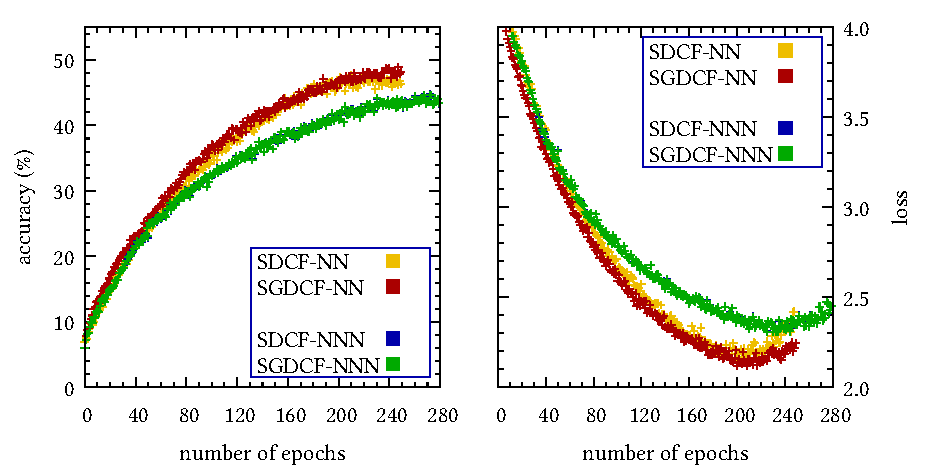
\includegraphics[width=1.1\textwidth]{./experiments/image-classification/comparison-token-mixers/graph-conv/graph-conv.pdf}}
    \caption{
        Comparison of the behavior of the traditional convolution based conformers (yellow and blue) to the graph based ones for image training data.
        The Blue and the green curve are completely identical (but calculated by optimizing different models), therefore blue is not visible.
        The reason, why the red and yellow curve are not also identical is due to different uses of the random number generator.
    }
    \label{fig:graph-convolution-works}
\end{figure}

The data shows, that the implementations of SDCF-NNN and SGDCF-NNN behave exactly identical, even though they compute the path interactions with different operations, as they are mathematically identical.

One can expect, that SDCF-NN and SGDCF-NN behave likewise, but slight differences in the data of these two be observed.
This is because of the different ways, the pseudo random number generator of PyTorch is used:
\begin{sloppypar} % I hate to have to use this hack, but line-broken file paths look more ugly and are on top unreadable
    The implementation of the graph-convolution \phantom{asdasdasdasdasdasdasdasdasdasdasdasdasd}
        \makebox{(\texttt{GraphMaskConvolution} in \filepath{\cite{selfComputerScience}}{/models/metaformer.py})}
    and the conventional-convolution 
        \makebox{(\texttt{SymmDepthSepConv2d} in \filepath{\cite{selfComputerScience}}{/models/helpers/SymmConv2d.py})}
        \phantom{aa}
        query the random number generator a different number of times, because the graph implementation always allocates ($3 \cdot \mathrm{channels}$) weights and the conventional implementation only allocates ($2 \cdot \mathrm{channels}$) weights for nn interactions and ($3 \cdot \mathrm{channels}$) for nnn.
        This causes the random number generator to drift apart and produces a propagating difference in the calculations \emph{only} for nn and not for nnn.
\end{sloppypar}

While this is a fixable flaw of the implementation, it clearly shows that the graph and non-graph implementations are behaving similar, even if the starting conditions are non-equivalent.
The comparison among the whole set of metaformers will emphasize how similar these two curves really are.

This proves, that convolutions can directly be translated into a graph context and motivates their function on non-tensor-like data structures.\\

\FloatBarrier
The architectures are compared against each other in the last section discussing the first experiment. 
\autoref{table:overall-comparison-data} shows the one to one comparison of all implemented metaformer variations on the same task.
The hyperparameters (optimizer, batch size, embed dimension, depth, etc.) were \emph{exactly the same for all runs}. 
The complete course of the validation metrics for selected runs is printed in \autoref{fig:overall-comparison-data}.

As it is impossible to discuss all the collected data in depth, only the most interesting observations will be emphasized.
Several trends can be noticed across the whole metaformer lineup. 


\begin{table}[htbp]
    \centering
    \makebox[\textwidth][c]{
        \begin{tabular}{l|llllllll} 
            \toprule
            name & $\mathrm{acc}_\mathrm{max}$ & $\mathrm{ep}_\mathrm{max}$ & \#params & $t$ / ep & $t_\mathrm{max}$ & $\frac{t}{\mathrm{param}}$ & $\frac{t_\mathrm{max}}{\mathrm{acc}}$ & $\frac{\mathrm{param}}{\mathrm{acc}}$ \\
            \midrule 
            TF (learned) & \SI{51.30}{\percent}  & \SI{62}{} & \SI{5543332}{} & \SI{391.01}{\second} & \SI{6.73}{\hour} & \SI{1.00}{} & \SI{1.00}{} & \SI{1.00}{} \\
            TF (sinus) & \SI{51.03}{\percent}  & \SI{66}{} & \SI{5505700}{} & \SI{391.32}{\second} & \SI{7.17}{\hour} & \SI{1.01}{} & \SI{1.07}{} & \SI{1.00}{} \\
            TF (none) & \SI{49.11}{\percent}  & \SI{63}{} & \SI{5505700}{} & \SI{391.22}{\second} & \SI{6.85}{\hour} & \SI{1.01}{} & \SI{1.06}{} & \SI{1.04}{} \\
            GTF-NN (learned) & \SI{50.01}{\percent}  & \SI{80}{} & \SI{5543368}{} & \SI{435.25}{\second} & \SI{9.67}{\hour} & \SI{1.11}{} & \SI{1.47}{} & \SI{1.03}{} \\
            GTF-NN (sinus) & \SI{49.38}{\percent}  & \SI{68}{} & \SI{5505736}{} & \SI{435.53}{\second} & \SI{8.23}{\hour} & \SI{1.12}{} & \SI{1.27}{} & \SI{1.03}{} \\
            GTF-NN (none) & \SI{48.42}{\percent}  & \SI{80}{} & \SI{5505736}{} & \SI{435.73}{\second} & \SI{9.68}{\hour} & \SI{1.12}{} & \SI{1.52}{} & \SI{1.05}{} \\
            GTF-NNN (learned) & \SI{51.58}{\percent}  & \SI{75}{} & \SI{5543368}{} & \SI{435.27}{\second} & \SI{9.07}{\hour} & \SI{1.11}{} & \SI{1.34}{} & \SI{0.99}{} \\
            GTF-NNN (sinus) & \SI{49.87}{\percent}  & \SI{70}{} & \SI{5505736}{} & \SI{435.47}{\second} & \SI{8.47}{\hour} & \SI{1.12}{} & \SI{1.29}{} & \SI{1.02}{} \\
            GTF-NNN (none) & \SI{50.38}{\percent}  & \SI{79}{} & \SI{5505736}{} & \SI{434.84}{\second} & \SI{9.54}{\hour} & \SI{1.12}{} & \SI{1.44}{} & \SI{1.01}{} \\
            PF & \SI{46.39}{\percent}  & \SI{367}{} & \SI{3727012}{} & \SI{217.14}{\second} & \SI{22.14}{\hour} & \SI{0.83}{} & \SI{3.64}{} & \SI{0.74}{} \\
            GPF-NN & \SI{43.26}{\percent}  & \SI{403}{} & \SI{3727012}{} & \SI{213.39}{\second} & \SI{23.89}{\hour} & \SI{0.81}{} & \SI{4.21}{} & \SI{0.80}{} \\
            GPF-NNN & \SI{47.43}{\percent}  & \SI{432}{} & \SI{3727012}{} & \SI{213.40}{\second} & \SI{25.61}{\hour} & \SI{0.81}{} & \SI{4.11}{} & \SI{0.73}{} \\
            DCF & \SI{46.13}{\percent}  & \SI{96}{} & \SI{3747748}{} & \SI{317.41}{\second} & \SI{8.46}{\hour} & \SI{1.20}{} & \SI{1.40}{} & \SI{0.75}{} \\
            SDCF-NN & \SI{47.66}{\percent}  & \SI{210}{} & \SI{3731620}{} & \SI{319.98}{\second} & \SI{18.67}{\hour} & \SI{1.22}{} & \SI{2.98}{} & \SI{0.72}{} \\
            SDCF-NNN & \SI{44.49}{\percent}  & \SI{260}{} & \SI{3733924}{} & \SI{319.72}{\second} & \SI{23.09}{\hour} & \SI{1.21}{} & \SI{3.95}{} & \SI{0.78}{} \\
            SGDCF-NN & \SI{48.78}{\percent}  & \SI{237}{} & \SI{3731620}{} & \SI{250.64}{\second} & \SI{16.50}{\hour} & \SI{0.95}{} & \SI{2.58}{} & \SI{0.71}{} \\
            SGDCF-NNN & \SI{44.39}{\percent}  & \SI{260}{} & \SI{3733924}{} & \SI{280.66}{\second} & \SI{20.27}{\hour} & \SI{1.07}{} & \SI{3.48}{} & \SI{0.78}{} \\
            CF & \SI{50.50}{\percent}  & \SI{106}{} & \SI{7710628}{} & \SI{386.45}{\second} & \SI{11.38}{\hour} & \SI{0.71}{} & \SI{1.72}{} & \SI{1.41}{} \\
            \bottomrule
        \end{tabular}
    }
    \vspace{0.1cm}
    \caption{Tabular representation of the performance data for different metaformers in the image classification task.
            The columns from left to right are: maximum top-1-accuracy, epoch this max accuracy was reached, the number of trainable parameters, the time per epoch, the time until the maximum accuracy was reached, the calculation time per parameter factor, the time until the maximum accuracy was reached per maximum accuracy factor and the number of parameters per maximum accuracy factor.
            The three factors are scaled so that \emph{TF (learned)} corresponds to \SI{1.00}{}. For everything but $\mathrm{acc}_\mathrm{max}$ lower is better. The maximum accuracy and the corresponding epoch have been chosen manually to select values that take both the accuracy and the loss curves into account. Because of that, sometimes bigger accuracies are reached later than the ones listed in the table.
            But they were excluded as lucky outliers, if the loss was already signaling overfitting.
    }
    \label{table:overall-comparison-data}
\end{table}

\begin{figure}[p]
    \centering
    \vspace{-1cm}
    \makebox[1.04\textwidth][r]{
        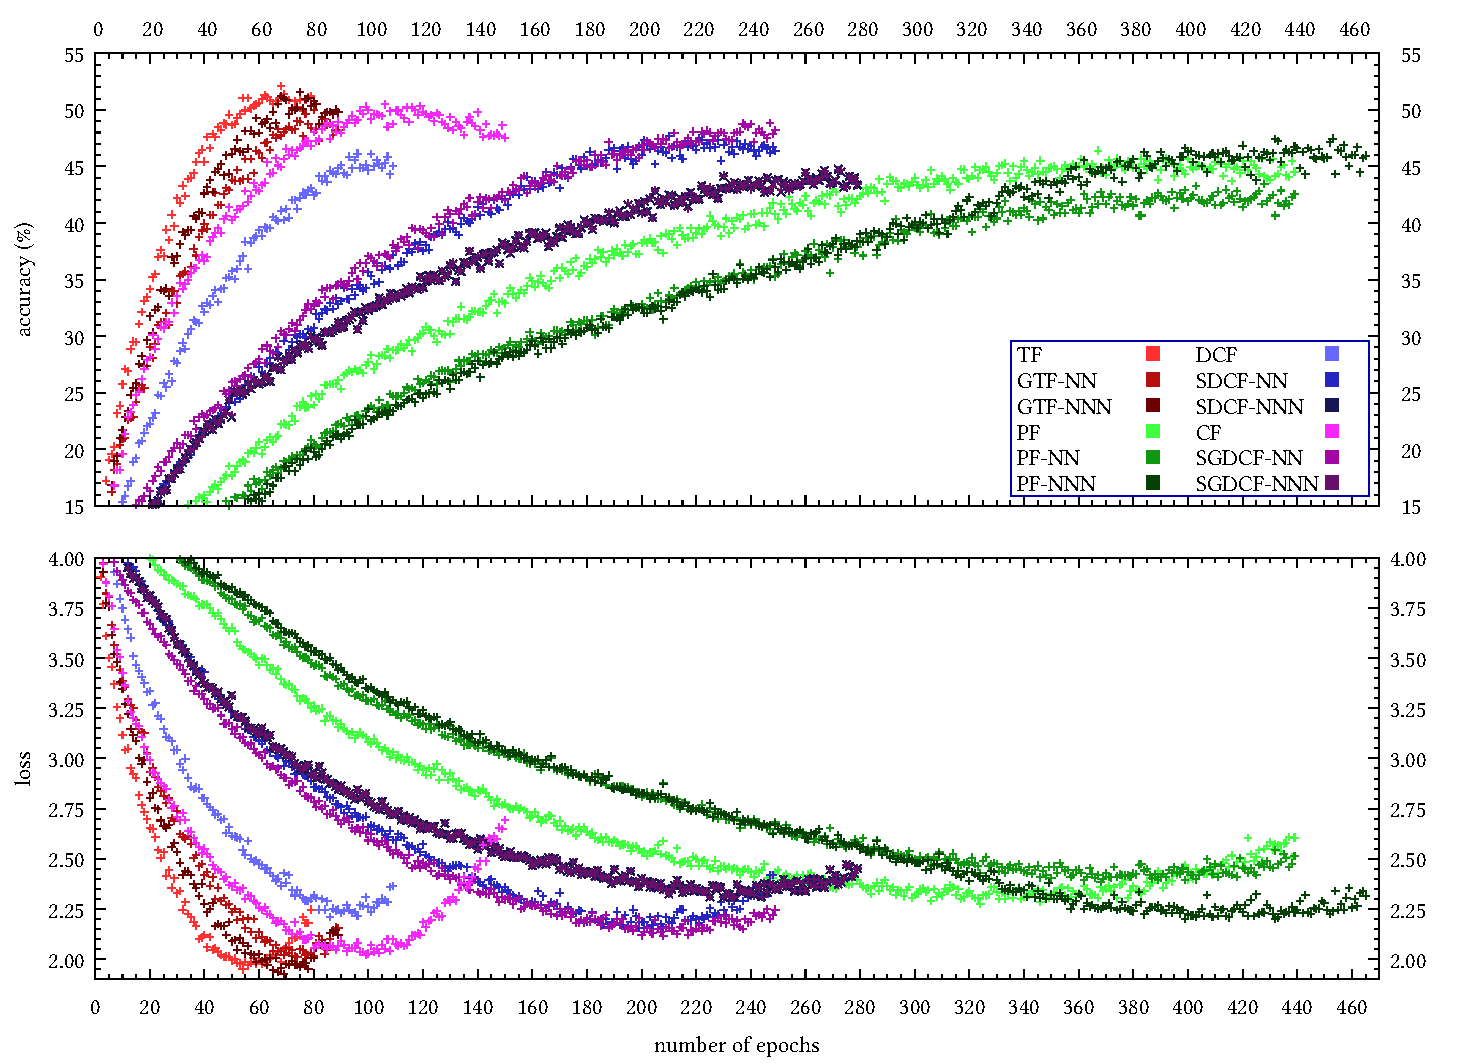
\includegraphics[width=\textheight,angle=90,origin=c]{./experiments/image-classification/comparison-token-mixers/overall-comp/overall-comp.pdf}
        }
    \caption{Graphic depiction of accuracy and loss of the metaformer architectures on the image classification task. 
            For the transformer architectures, only the \emph{learned} pe is drawn, as the other encodings are already printed in \autoref{fig:positional-encoding-training}. 
            This data is from the same runs as the data in \autoref{table:overall-comparison-data}.
    }
    \label{fig:overall-comparison-data}
\end{figure}

\paragraph{The attention based transformers} for the start score the highest overall accuracy. 
The graph-masked attention falls only slightly behind the full transformer in the case of the nn-limited attention and even pulls ahead in some of the positional encodings in the case of the nnn-limited interaction.
All the models are basically identical in terms of required parameters, only the learned pe requires a noticeable different amount of weights as already discussed in \autoref{sec:experiments-positionalencoding}. 
The weights inside the graph masks are basically negligible.

Contrary large discrepancies occur in the overhead in computational time.
The graph variants require both more epochs to achieve maximum accuracy, as well as the epochs itself taking longer to be calculated.
Both is sensible, as the masking requires extra calculations and the zeroing of interactions creates a \emph{choke point} for the backpropagating information (this will become even more pronounced in the later architectures). 
Still it is clear, that masking attention does not hurt the performance as much as one could expect (the defining characteristic of the attention module being the \emph{global} interaction range, that is here taken away).

As the nn-graph-attention takes both longer to train and achieves less accuracy than the nnn-graph-attention, using the latter only brings advantages for the image classification task.
That the nnn variant even outperforms the full transformer in terms of raw accuracy can probably be attributed to the relatively small model size and un-optimized training procedure.
As a perfectly trained full transformer should be able to replicate a graph transformer, this shows that while in theory the latter is inferior, in practice for small models or imperfect training procedures it can definitely be beneficial to force the inductive bias of \emph{locality} upon the model.

A so far unmentioned detail could furthermore vastly improve the graph-transformers. 
This will be discussed in \autoref{sec:experiments-efficiency-graphs}.

\paragraph{The convolution based conformers} continue all the described trends.
They require less trainable weights (around \SI[]{33}[]{\percent} less) than the transformers.
Their maximum accuracy is slightly worse than the transformers', and they require longer to reach peak accuracy.
Though as soon as they are fully trained, they can both be evaluated quicker and have a overall smaller footprint due to the smaller weight count.
This shows, that for our small size of network, shaping a model around a hard coded inductive bias takes more effort, but can pay of in terms of efficiency.

Interestingly, when comparing the symmetric and non-symmetric variants, the non-symmet\-ric one converges \emph{significantly} faster in training (by a factor of \SIrange[]{2.1}{2.7}{}). 
This can again be attributed to the strict choke point of only two weights for SDCF-NN in comparison to the nine inside the DCF kernel.

It is however very interesting to see, that the conformer architecture is the only kind of metaformer where the nn-convolution performed better than the nnn variant and the full variant, by a very significant margin of \SI[]{4.2}[]{\percent}.
This shows that it is clearly worthwhile to experiment with different interaction schemes, when employing graph networks.

As previously discussed, the traditional convolution and graph convolution variations are equivalent on tensor data.
The models clearly show this, especially when comparing the course of the curves in \autoref{fig:overall-comparison-data}.
Unexpected on the other hand is the significantly worse performance of the traditional variant in terms of computational speed (\SIrange{13}{27}{\percent} longer time per epoch).
This may seem counter intuitive, but can be explained when looking at the implementation. 
As all the models use the same underlying framework, the internal representation is always stored as $b \times (n=w\cdot h) \times e$, with the batch dimension $b$, the number of patches $n$, the width and height in patches $w$ and $h$ and the embed dimension $e$. 
When a traditional convolution should get applied, this needs to be reshaped to correspond to $b \times e \times w \times h$ and reversed after the convolution operation. 
This step creates an unnecessary overhead, that could be left out, if only traditional convolutions were needed.

\paragraph{The pooling based poolformers} sit at the opposite end of the overall trends.
They require the least amount of parameters and - because of the very loose coupling of the pooling operation - the by far longest time to train.
A fully trained poolformer though provides both the best parameters per accuracy efficiency, as well as the lowest evaluation time.
PF and GPF-NNN being practically identical, which was expected on tensor data.

The overall accuracy is definitely lower, than that of a transformer, but because of the significant efficiency advantage, the poolformer's performance is still definitely competitive.

\paragraph{The full conformer} is listed in the lineup, but it - as already discussed - can not be considered a \emph{strict} metaformer.
The performance is relatively high and the speed of convergence is average. 
Though the extremely large parameter count (more than \SI[]{106}[]{\percent} \emph{more} than a depthwise conformer) drives the point why depthwise separable convolutions are so desirable in the metaformer framework and beyond.
